\thispagestyle{endchapter}

\begin{tcolorbox}

\vspace{80pt}
	\lettrine{I}{n} summary, Migovec now has three major systems and over a dozen smaller
caves in active exploration. The exploration in \passage{Vrtnarija} was at
the very end of our endurance limits - the minimal trip length to
achieve anything was 15hrs. Our plans are to camp down there in 2009 in
order to have far more man hours at the `coal face' and to offer the
psychological and physiological refuge of a camp in a location that, in
spite of its relatively shallow depth, is truly a long way from a safe
place.

The mountain is unique in having such complicated Alpine cave formation
at various depths, and now constitutes 21.988 km of passage beneath just
a square kilometre of surface.

Everything newly explored was surveyed to BCRA Grade 4b. Underground
photography as part of documentation took place in \passage{Vrtnarija}, \passage{E1},
\passage{Plopzilla} (in \passage{Sistem Mig}) and \passage{Planika Jama}. We were limited by
there being only one underground photographer on the expedition.

A new survey on an East-West projection has been drawn of \passage{M2} and
\passage{Vrtnarija}.
 
The weekend after the expedition van headed home, a small Slovene /
English team went back down \passage{M2} armed with an enormous drill \&
battery. With 6 shot holes they blew their way through the rift, to the
head of a short pitch.

This was returned to in October 2008, and dropped - all the new finds in
\passage{M2} being surveyed at the same time. The new pushing front is
another, almost impenetrable rift, and a climb up into a series of tight
phreatic passage. The survey data indicates that \passage{M2} itself is
trending away from \passage{Captain Kangaroo}.

During the expedition a major error was discovered in our survey data - namely that the wrong \passage{M2} entrance (there are two, separated by 25 m horizontal) was connected into the surface survey. This caused a jump in the position of the bottom of \passage{M2}, taking it further from \passage{Vrtnarija}.

With the corrected data, our closest approach is now 23 m between the
large chamber found below \passage{Cheesecake} and the confluence at the end of
\passage{M2}.

\end{tcolorbox} 
	\backgroundsetup{	scale=1,
					color=black,
					opacity=1,
					angle=0,
					contents={%
							  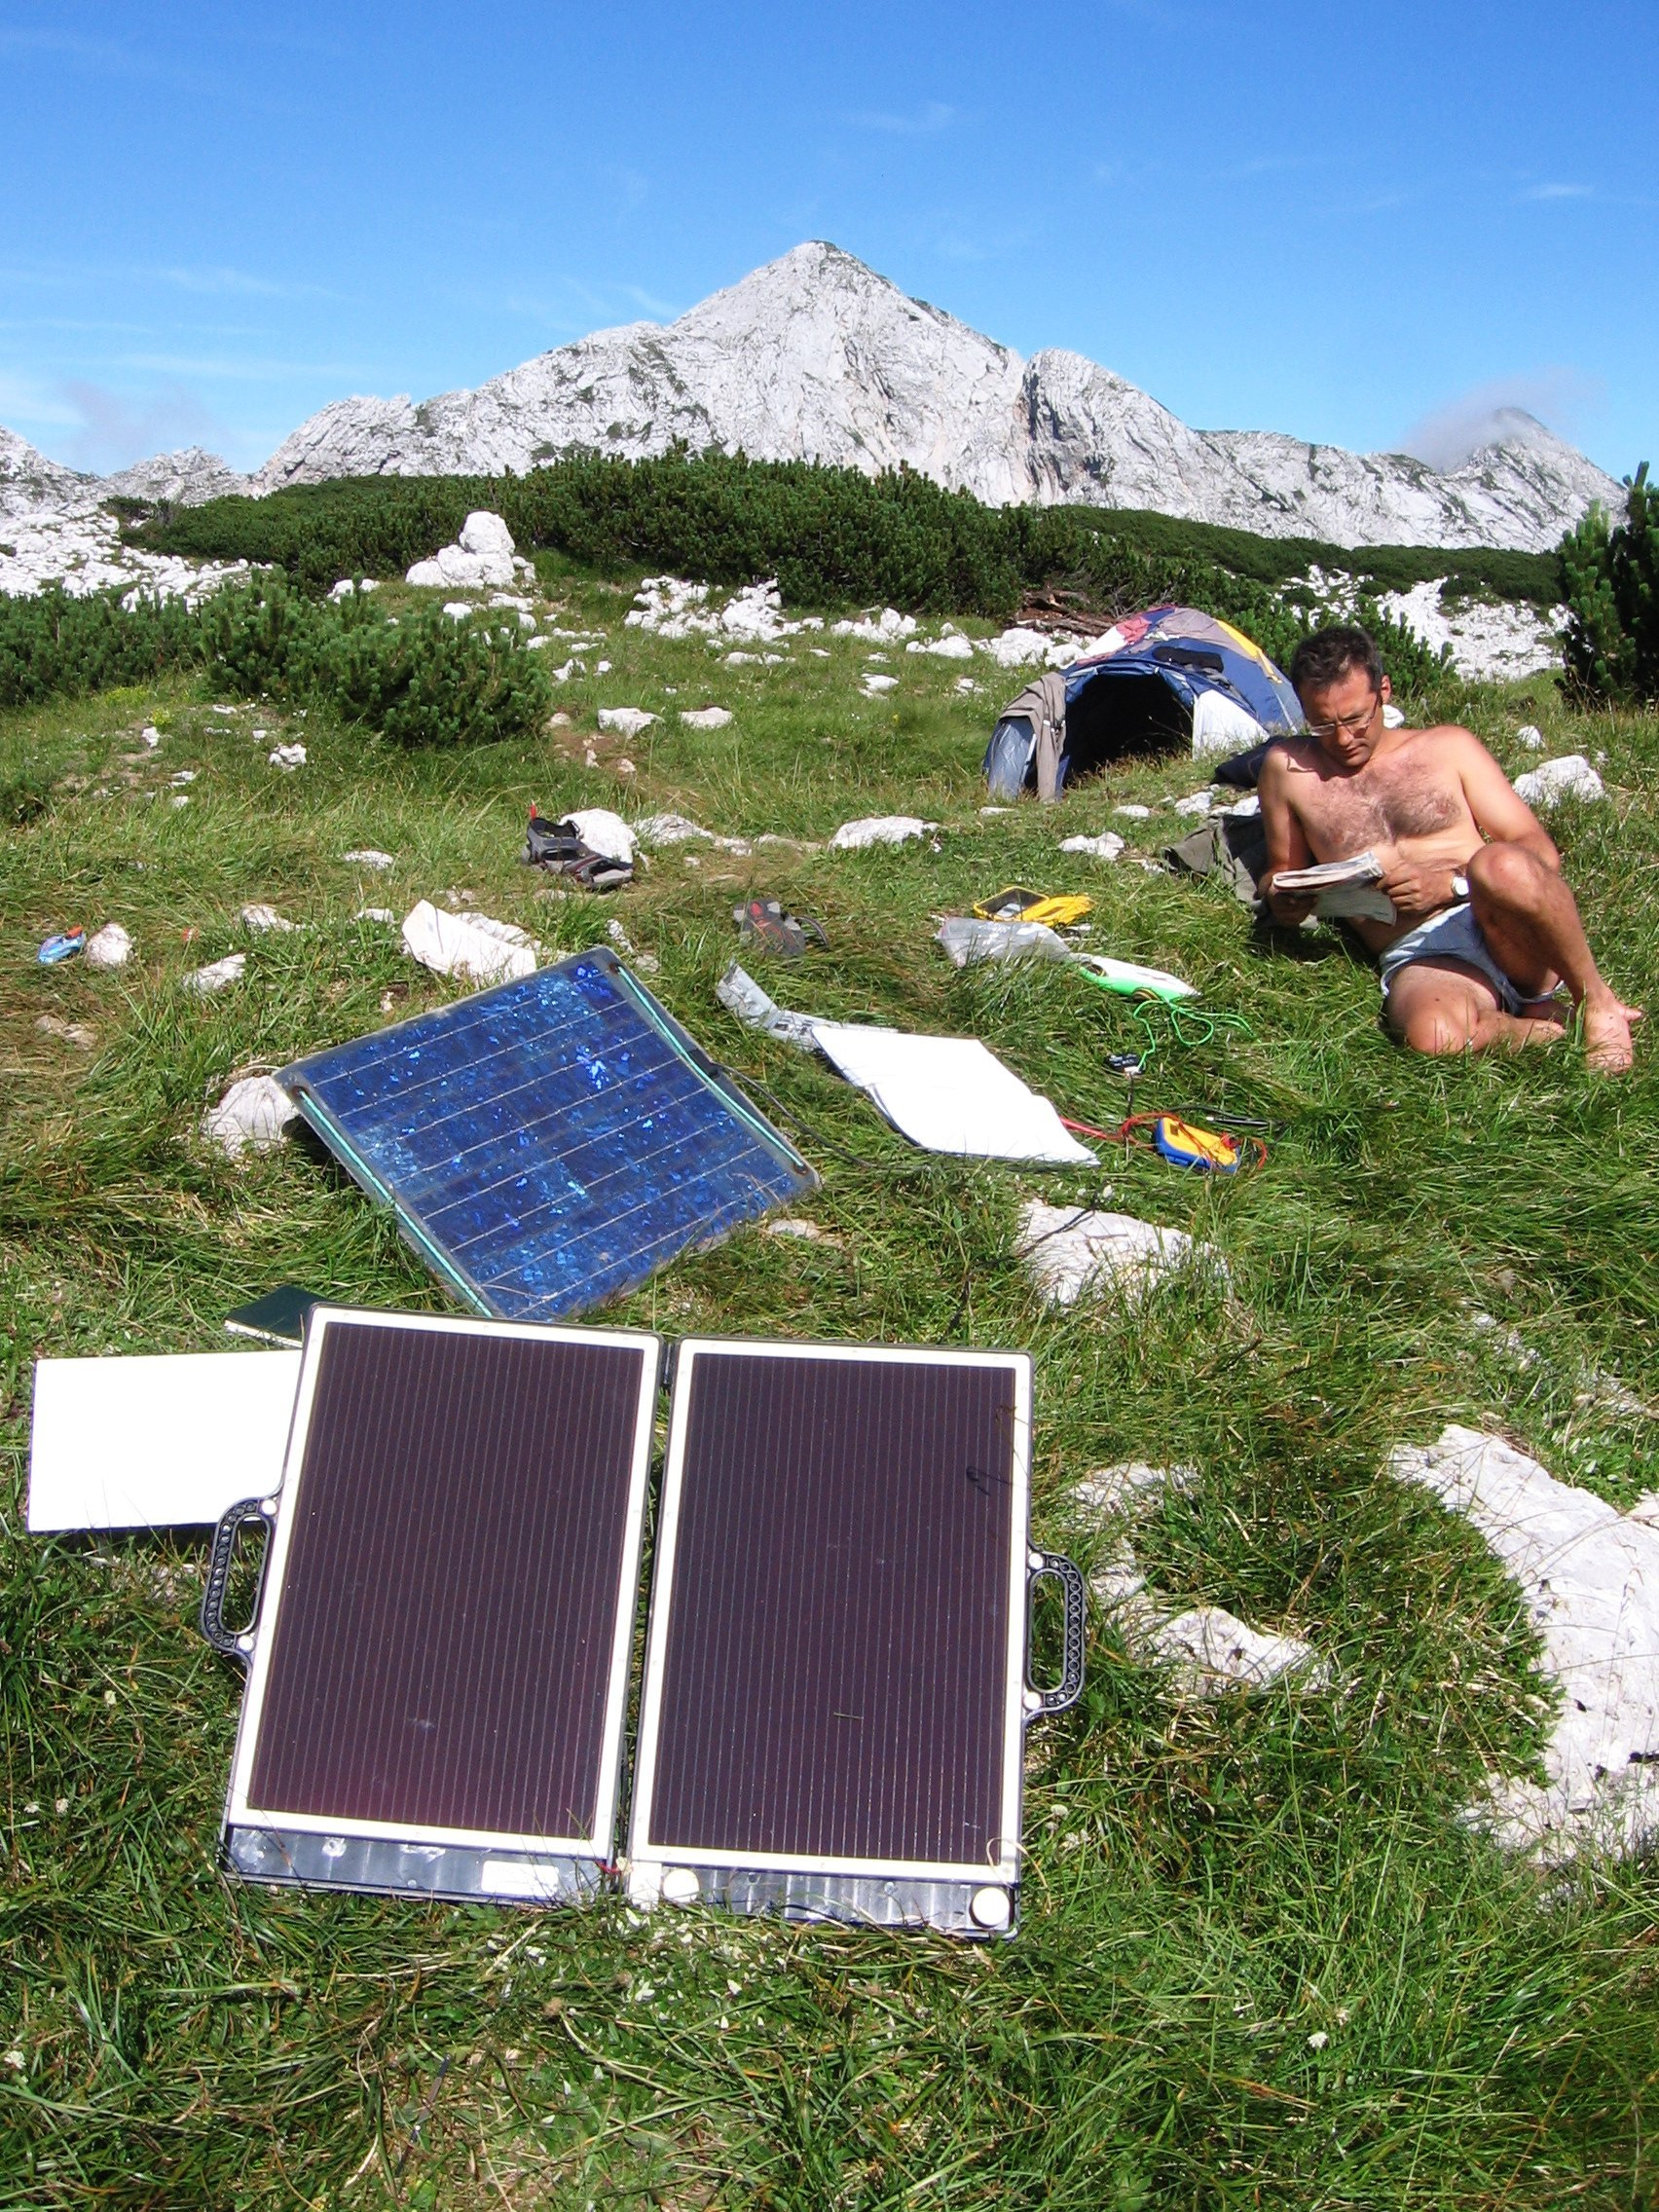
\includegraphics[height=\paperheight]{2008/outro/Jarvist Frost - canon a520 - both solar panels with skrbina in the background--orig.jpg}
 					}
	}
\BgThispage
